\subsection{Development Board}

The development board for this project is the Raspberry Pi 4 Model B, shown in figure \ref{fig:rasp}, considering it is one of the constraints identified in the analysis phase (\ref{subsection:requirements_constraints}). This board includes a 64-bit quad-core ARM processor, the BCM2711, multimedia and connection features, ressembling to a computer-like board that serves multiple applications. The following list shows the Raspberry Pi 4 Model B main features:

\begin{itemize}
        \item 2GB LPDDR4-3200 SDRAM;
        \item 2.4 GHz and 5.0 GHz IEEE 802.11ac wireless, Bluetooth 5.0, BLE;
        \item Raspberry Pi standard 40 pin GPIO header;   
        \item 2 USB 3.0 ports and 2 USB 2.0 ports;
        \item 2 micro-HDMI ports;
        \item 1 display port (2-lane MIPI DSI);
        \item 1 camera port (2-lane MIPI CSI);
        \item 1 jack 3,5 mm port (4-pole stereo audio and composite video port);
		\item graphic support (OpenGL ES 3.1, Vulkan 1.0);
		\item Micro-SD card slot.
\end{itemize}

The Raspberry Pi 4 Model B is used as a development board for this project, as it would not be used in a final application because not all its features are used. So, in a final application, the development board would be chosen based on the features nedded or would be designed.

% A raspberry é apenas uma board de desenvolvimento, não é o hw que usariamos numa aplicação final.

\begin{figure}[H]
	\centering
	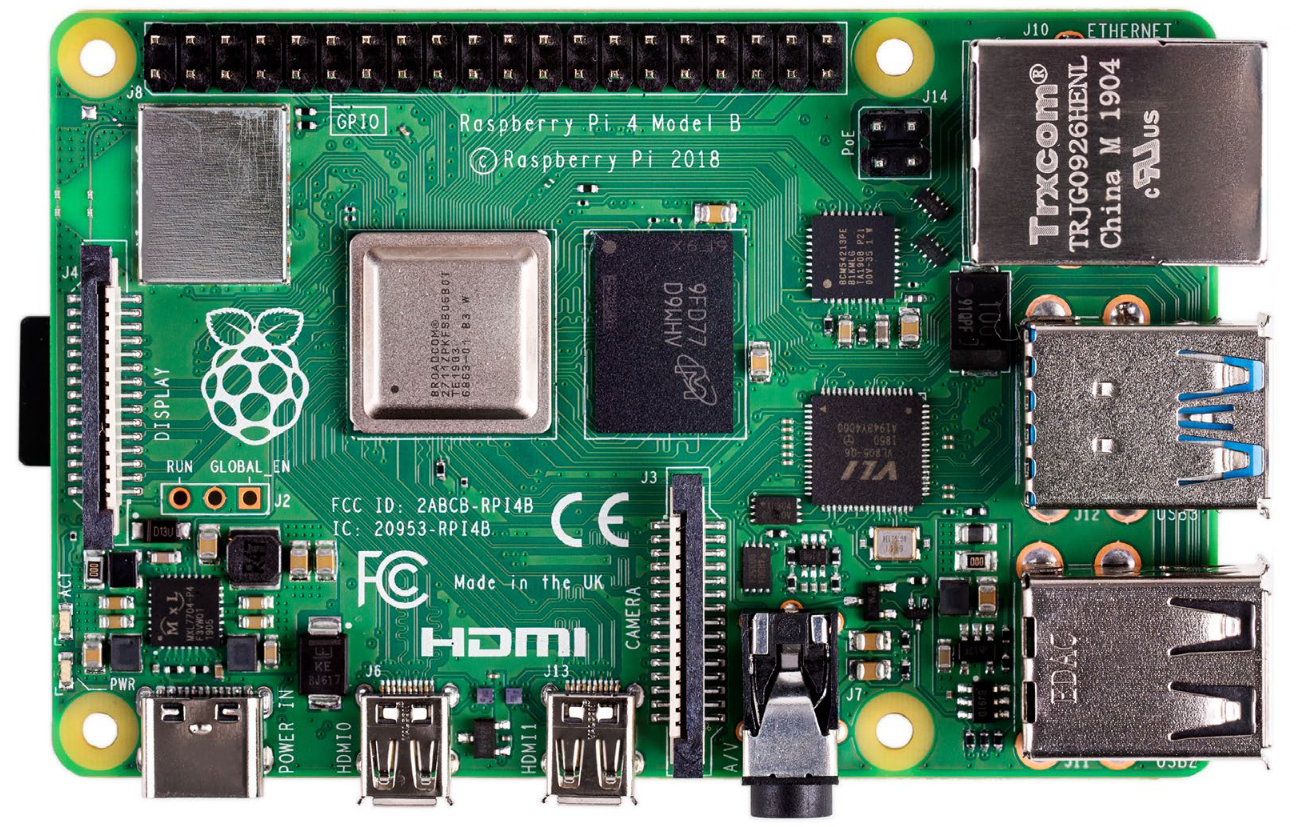
\includegraphics[width=.75\textwidth]{07hw_specification/raspberryPi}
	\caption{Raspberry Pi 4 Model B.}
	\label{fig:rasp}
\end{figure}

%**********************************************************
\myparagraph{\ac{gpio}}

The Raspberry Pi 4 Model B board comes with a standard 40 pin GPIO header, that allows to interface with external peripherals. This GPIO also provides some interface technologys, like UART, I2C or SPI. The GPIO pinout of this board is shown in figure \ref{fig:rasp_pinout} \cite{pinout}.

\begin{figure}[ht]
	\centering
	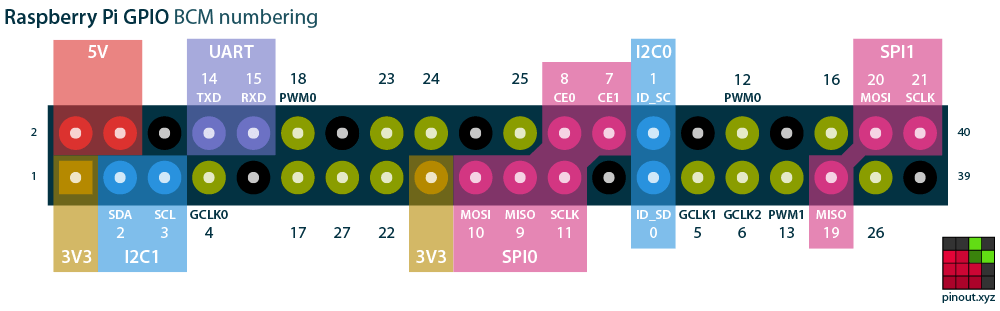
\includegraphics[width=1\textwidth]{07hw_specification/raspberryPi_pinout}
	\caption{Raspberry Pi 4 Model B GPIO Pinout.}
	\label{fig:rasp_pinout}
\end{figure}

%**********************************************************
\subsection{Lamp}

In order to light the streets efficiently, we use a LED lamp, that is the type of lamps with the better energy efficienty. It must be an adjustable lamp to control the lasmp brightness, so the lamp selected was a G4 socket 12 V AC/DC LED lamp. The lamp is controled using a driver, that is aproached in subsection \ref{subsection:driver} the that takes a \ac{pwm} signal (Pin 18) from the Raspberry Pi as input. 

\begin{figure}[ht]
	\centering
	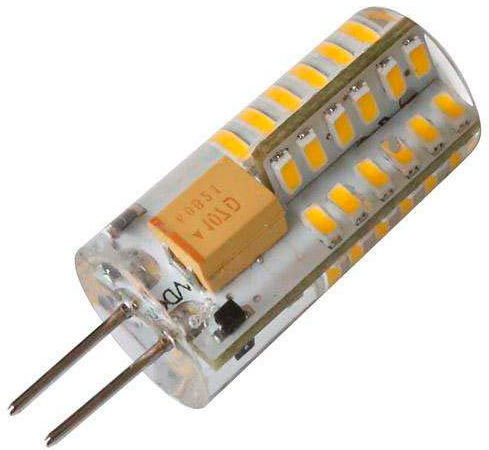
\includegraphics[width=1\textwidth]{07hw_specification/lamp}
	\caption{LED Lamp.}
	\label{fig:lamp}
\end{figure}

\myparagraph{Characteristics}

\begin{itemize}
	\item Power supply: DC 12 V;
	\item Eletric power: 2 W;
	\item Adjustable;
	\item Socket: G4;   
	\item Chip controller: SMD3014.
\end{itemize}

In a real-scale project, it would be used a different lamp, with supplu voltage of 230 V AC and other specific characteristics  like  rate, in  from water and dust (IP65 \ref{ip65}). It would be also used a LED lamp with higher eletric power. 

%**********************************************************
\subsection{Luminosity Sensor}

In order to know when is night time, that is, when the light conditions are low, one needs to determine the ambient light conditions. To do that, it is used a digital ambient light sensor, the TSL2581 \cite{light_sensor}, represented in \ref{fig:light_sen}. It was chosen this project because this sensor communicates with the Raspberry Pi using \ac{i2c} communication protocol, so it gives a digital value of the lumminusity, according to the light conditions, so it isn't necessary to calibrate this sensor (with a potenciometer, for example) when installing a new local system.

\begin{figure}[ht]
	\centering
	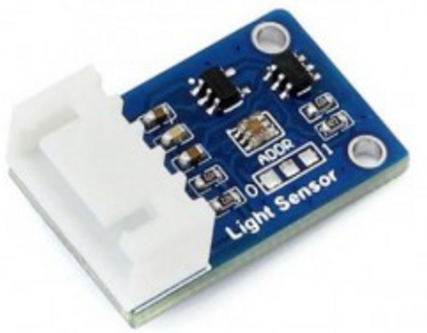
\includegraphics[width=0.60\textwidth]{07hw_specification/light_sen}
	\caption{TSL2581 Light Sensor.}
	\label{fig:light_sen}
\end{figure}

\paragraph*{Characteristics}
\begin{itemize}
	\item \ac{i2c} interface directly outputs the ambient light intensity value;
	\item High precision output, with an infrared photodiode;
	\item Allows connection to 3,3 V or 5,5 V MCU systems;
	\item 16-bit resolution.
\end{itemize}

In the table \ref{table:light_sen} is shown the TSL2581 interface pins, being the \textit{SDA} pin used for data transfer, the \textit{SCL} pin used for clock synchronisation and the \textit{INT} pin used for interrupt output. 

\begin{table}[H]
	\centering
	\begin{tabular}{|m{5cm}|m{6cm}|}
		\hline
		\textbf{TSL2581 Pin} & \textbf{Board Pin}\\\hline\hline
		VCC & Pin 1 (3,3) V\\\hline
		GND & Pin 6 (GND)\\\hline
		SDA & Pin 2 (SDA)\\\hline
		SCL & Pin 3 (SCL)\\\hline
		INT & -\\
		\hline
	\end{tabular}		
	
	\caption{Light Sensor TSL2581 Interface Pins.}
	\label{table:light_sen}
\end{table}

\myparagraph{Test Cases}
It is important to know how the light sensor works, and how it will behave upon certain events. In table \ref{table:test_light_sen} are shown test cases to this module.

\begin{table}[H]
	\centering
	\resizebox{\columnwidth}{!}
	{
		\begin{tabular}{|m{3cm}|m{5cm}||m{5cm}|}
			\hline
			\textbf{Test Case} & \textbf{Expected Output} & \textbf{Real Output}
			\\\hline\hline
			Read ambient luminosity & Return ambient luminosity  & -
			\\\hline
		\end{tabular}
	}
	\caption{Test Cases: TSL2581.}
	\label{table:test_light_sen}
\end{table}

%**********************************************************
\clearpage
\subsection{Motion Detector}
To know when to turn on the light, it is necessary to detect movement in the streets. For this project it is used a motion detector, more specifically a \ac{pir} sensor. The chosen sensor for this purpose was the PIR HC-SR501 \cite{pir}.

\begin{figure}[H]
	\centering
	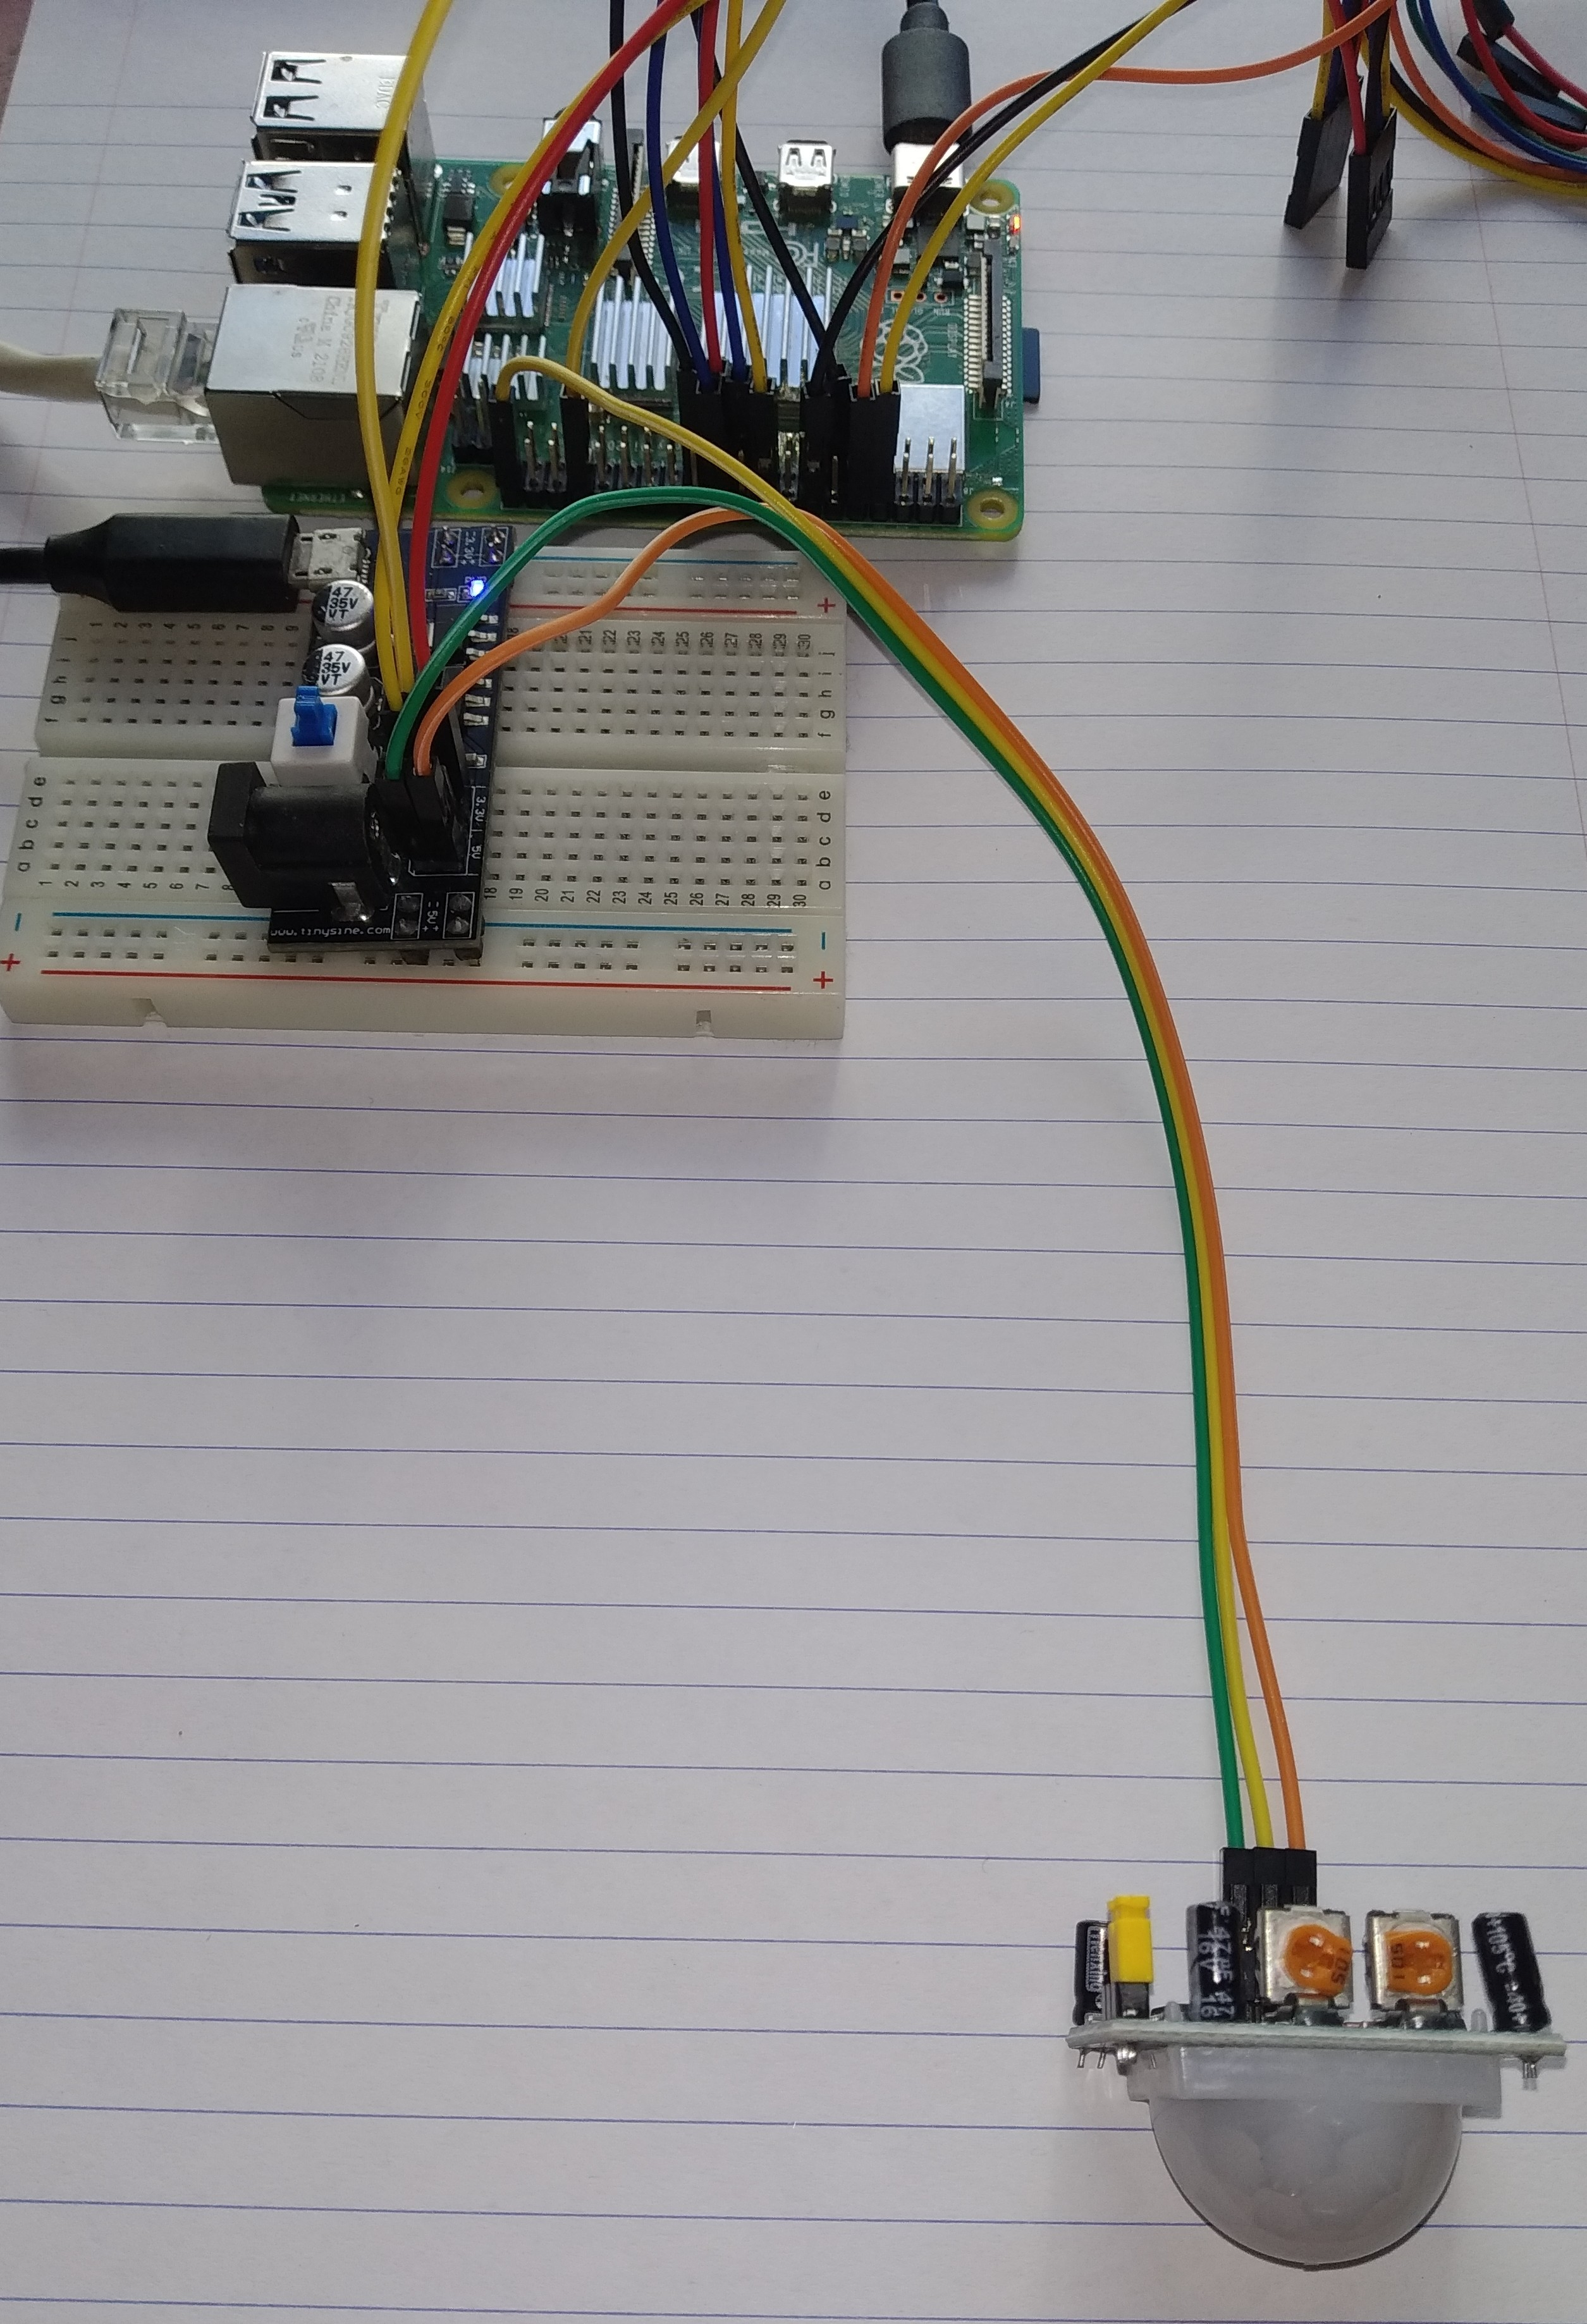
\includegraphics[width=0.70\textwidth]{07hw_specification/pir}
	\caption{PIR HC-SR501.}
	\label{fig:pir}
\end{figure}

\paragraph*{Characteristics}
\begin{itemize}
	\item Supply voltage range of 4,5 - 20 V;
	\item Static current: 50 uA;
	\item Detection range of 7 meters;
	\item Detection angle of 110 degrees;
	\item Two potenciometers to adjust the trigger sensitivity and the delay of the trigger signal, between 0,3 seconds and 5 minutes;
\end{itemize}

In the table \ref{table:pir} is shown the PIR HC-SR501 interface pins, being the output signal the pin SIGNAL. When no movement is detected, the sensor output is low (0,3~V), and when movement is detected, the sensor SIGNAL is high (5~V). 

\begin{table}[H]
	\centering
	\begin{tabular}{|m{5cm}|m{6cm}|}
		\hline
		\textbf{PIR HC-SR501 Pin} & \textbf{Board Pin}
		\\\hline\hline
		
		VCC & Pin 2(5 V)\\\hline
		SIGNAL & Pin 27\\\hline
		GND & Pin 6(GND)\\
		\hline
	\end{tabular}
	
\caption{PIR HC-SR501 Interface Pins.}
\label{table:pir}
\end{table}

\myparagraph{Test Cases}
It is important to know how the motion detector module works, and how it will behave upon certain events. In table \ref{table:test_pir} are shown test cases to this module.

\begin{table}[H]
	\centering
	\resizebox{\columnwidth}{!}
	{
		\begin{tabular}{|m{3cm}|m{5cm}||m{5cm}|}
			\hline
			\textbf{Test Case} & \textbf{Expected Output} & \textbf{Real Output}
			\\\hline\hline
			Movement in front of the sensor & Pin SIGNAL high (5 V) & -
			\\\hline
			No movement in front of the sensor & Pin SIGNAL low (0,3 V) & -
			\\\hline
		\end{tabular}
	}
	\caption{Test Cases: PIR HC-SR501.}
	\label{table:test_pir}
\end{table}

%**********************************************************
\subsection{Lamp Failure Detector}
In order to know when the lamp is broken, one needs to use a lamp failure detector, so it was designed a circuit represented in figure \ref{fig:failure_circuit}. 
%When the lamp  

\begin{figure}[H]
	\centering
	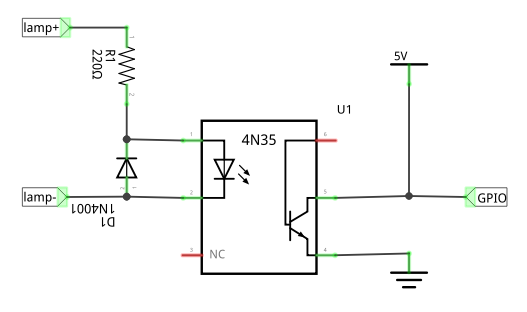
\includegraphics[width=0.6\textwidth]{07hw_specification/failure_schem}
	\caption{Lamp Failure Detector Circuit.}
	\label{fig:failure_circuit}
\end{figure}

The optocoupler chosen was the 4N35 \cite{4n35}, represented in figure \ref{fig:failure}

\begin{figure}[H]
	\centering
	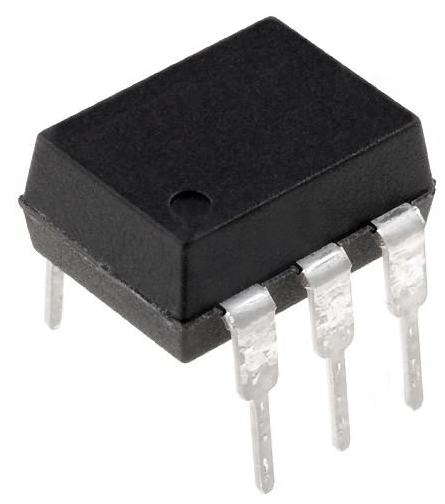
\includegraphics[width=0.4\textwidth]{07hw_specification/failure}
	\caption{Optocoupler 4N35.}
	\label{fig:failure}
\end{figure}

%**********************************************************
\subsection{Camera}
In order to the detection of available parking spots, it's used a camera, as shown in figure \ref{fig:camera}. This is the Raspberry Pi Camera Module V1, capable of delivering a clear 5 MP resolution image, or 1080p HD video recording at 30fps. \cite{camera}

\begin{figure}[H]
	\centering
	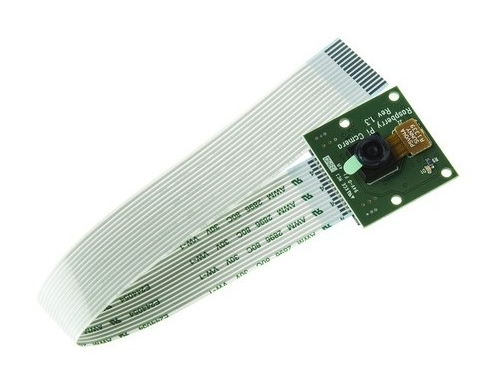
\includegraphics[width=0.6\textwidth]{07hw_specification/camera}
	\caption{Raspberry Pi Camera Module V1.}
	\label{fig:camera}
\end{figure}

\paragraph*{Characteristics}
\begin{itemize}
	\item 5MP OmniVision 5647 sensor;
	\item Fixed focus lens onboard;
	\item Still Picture Resolution: 2592 x 1944;
	\item 15-pin ribbon cable, to the dedicated 15-pin MIPI \ac{csi};
	\item Video recording: Supports 1080p @ 30fps, 720p @ 60fps.
\end{itemize}

\clearpage
\myparagraph{Connection scheme}
This device plugs directly into the \ac{csi} connector on the Raspberry Pi, as shown in figure \ref{fig:connect_camera}, through the use of a 15-pin ribbon cable.

\begin{figure}[ht]
	\centering
	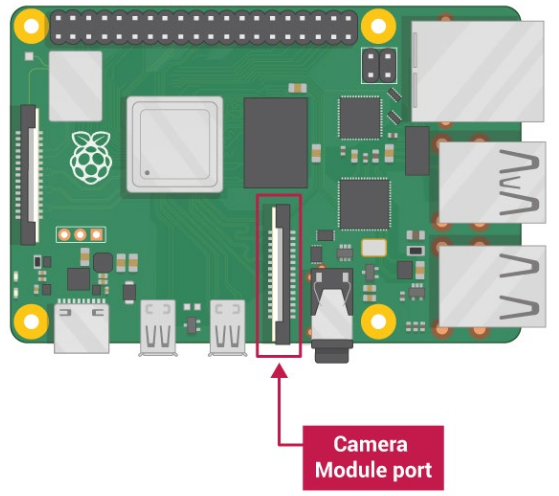
\includegraphics[width=0.60\textwidth]{07hw_specification/connect_camera}
	\caption{Connection scheme: Camera Module.}
	\label{fig:connect_camera}
\end{figure}

\myparagraph{Test Cases}
It is important to know how the camera module will behave upon certain events. In table \ref{table:test_camera} are shown test cases to this module.

\begin{table}[H]
	\centering
	\resizebox{\columnwidth}{!}
	{
	\begin{tabular}{|m{3cm}|m{5cm}||m{5cm}|}
		\hline
		\textbf{Test Case} & \textbf{Expected Output} & \textbf{Real Output}
		\\\hline\hline
		Take picture & Clear output image & -
		\\\hline
	\end{tabular}
	}
	\caption{Test Cases: Camera Module.}
	\label{table:test_camera}
\end{table}


%**********************************************************
\clearpage
\subsection{LoRa Module}
To allow each local system to communicate to the gateway, and vice-versa, it's used LoRa communication technology, requiring for that LoRa Modules, as the one presented in figure \ref{fig:lora_module}. This module, from Ai-Thinker company, uses SX1278 \ac{ic} from SEMTECH, and works on a 433~MHz frequency, with a range up to 10 km in line of sight. \cite{sx1278} \cite{lora_module}

\begin{figure}[H]
	\centering
	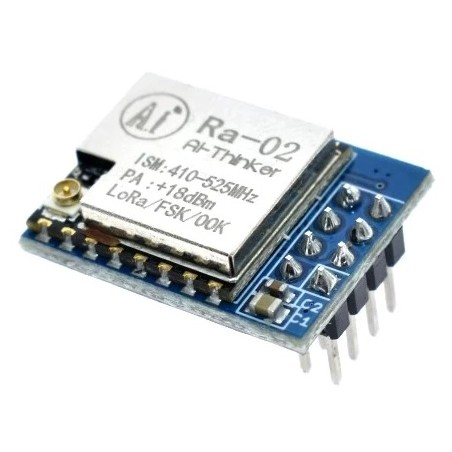
\includegraphics[width=0.5\textwidth]{07hw_specification/lora_module}
	\caption{LoRa Module SX1278 RA-02 433 MHz.}
	\label{fig:lora_module}
\end{figure}

\paragraph*{Characteristics}
\begin{itemize}
	\item LoRa modulation technology (Supports also FSK, GFSK, MSK, GMSK and OOK modulation modes);
	\item Effective Bitrate : 0,018 - 37,5 kbps;
	\item Payload length: 64 bytes;
	\item Half-duplex SPI communication;
	\item Programmable bit rates up to 300kbps;
	\item Packet engine with CRC up to 256 bytes;
	\item Male U.FL connector to support using of external RF antenna - Diameter: 15,5mm.
\end{itemize}

\begin{table}[H]
	\centering
		\begin{tabular}{|m{5cm}|m{6cm}|}
			\hline
			\textbf{SX1278 RA-02 Pinout} & \textbf{Description}
			\\\hline\hline
		
			VCC & Power in - 3,3 V\\\hline
			GND & Ground\\\hline
			RST & Reset \\\hline
			SCK & SPI clock input\\\hline
			NSS & SPI selected-IN\\\hline
			MISO & SPI data output\\\hline
			MOSI & SPI data input\\\hline
			DIO0 & Digital Input/Output Pin 0\\\hline
			\hline
		\end{tabular}
	
	\caption{LoRa Module SX1289 RA-02 Pinout Description.}
	\label{table:lora_module_pinout}
\end{table}

In order to achieve longer range and better signal quality in LoRa communication, an antenna may be used, as the one shown in figure \ref{fig:lora_antena}. RF antennas play a critical role in diverting, directing or concentrating radio wave transmission in a particular direction. 

%Antennas that have high gain will enable one to achieve longer range and better signal quality in LoRa communication, but must be aimed specifically in the direction of the receiving antenna. 

\begin{figure}[H]
	\centering
	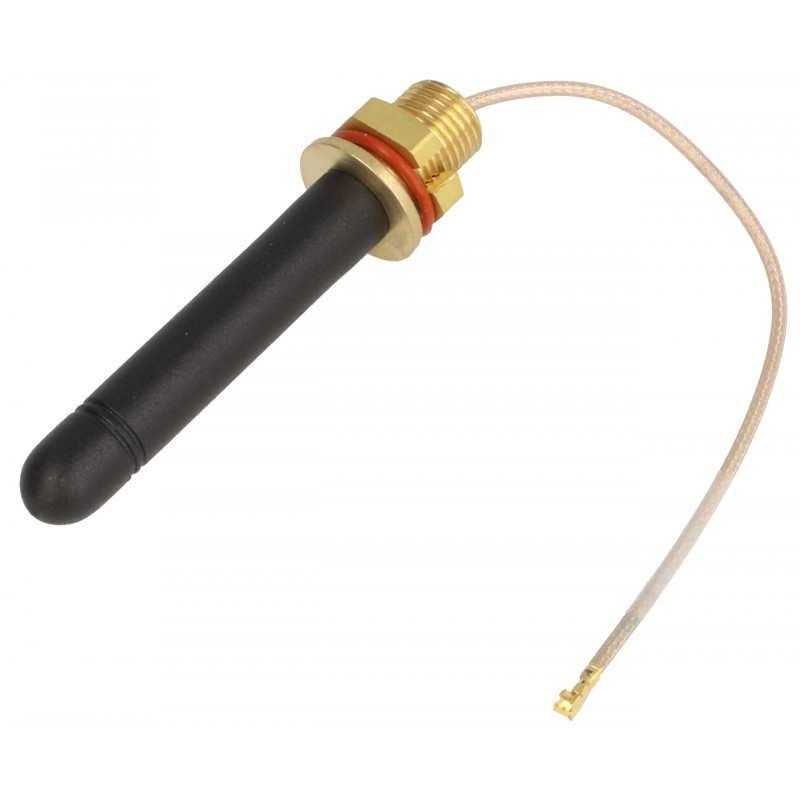
\includegraphics[width=0.40\textwidth]{07hw_specification/lora_antena}
	\caption{RF Antenna 433 MHz.}
	\label{fig:lora_antena}
\end{figure}

\paragraph*{Characteristics}
\begin{itemize}
	\item Frequency: 433,05 - 434,79 MHz;
	\item Antenna gain: 2 dBi;
	\item Connector I-PEX (U.FL) - Diameter: 15,5mm;
	\item Impedance 50 $\Omega$.
\end{itemize}

\myparagraph{Connection scheme}
In table \ref{table:connect_lora} it is shown the connection scheme of the LoRa module to the Raspberry Pi (remember figure \ref{fig:rasp_pinout}). Keep in mind that the RF antenna is directly connected to the LoRa module through an U.FL connector.

\begin{table}[H]
	\centering
	\begin{tabular}{|m{5cm}|m{6cm}|}
		\hline
		\textbf{SX1278 RA-02 Pin} & \textbf{Raspberry Pi Pin}
		\\\hline\hline
		
		VCC & 3,3 V
		\\\hline
		GND & GND
		\\\hline
		RST & GPIO 4
		\\\hline
		SCK & CLK
		\\\hline
		NSS & SPI0 CE0
		\\\hline
		MISO & SPI0 MISO
		\\\hline
		MOSI & SPI0 MOSI
		\\\hline
		DIO0 & GPIO 17
		\\\hline
	\end{tabular}
	
	\caption{Connection scheme: LoRa Module.}
	\label{table:connect_lora}
\end{table}

\myparagraph{Test Cases}
It is important to know how the LoRa module works, and how it will behave upon certain events. In table \ref{table:test_lora} are shown test cases to this module.

\begin{table}[H]
	\centering
	\resizebox{\columnwidth}{!}
	{
		\begin{tabular}{|m{3cm}|m{5cm}||m{5cm}|}
			\hline
			\textbf{Test Case} & \textbf{Expected Output} & \textbf{Real Output}
			\\\hline\hline
			Establish connection & Stable connection established & -
			\\\hline
			Send data & Data sent correctly & -
			\\\hline
			Receive data & Data received correctly & -
			\\\hline
		\end{tabular}
	}
	\caption{Test Cases: LoRa Module.}
	\label{table:test_lora}
\end{table}

%**********************************************************

\subsection{Driver}
\label{subsection:driver}
In order to control the lamp brightness through a GPIO pin from the Raspberry Pi, it's needed a driver circuit, as shown in figure \ref{fig:driver}. This circuit takes as input a \ac{pwm} signal, provided by the raspberry Pi, and also the power for the lamp, \(V_{CL}\), which comes directly from the power supply 12 V \ac{dc} output of the power module. The output of this circuit, the lamp voltage \(V_{L}\), is directly related to it's brightness, which one wants to control.

\begin{figure}[H]
	\centering
	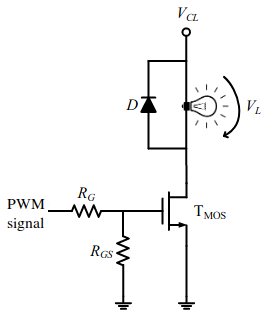
\includegraphics[width=0.5\textwidth]{07hw_specification/driver}
	\caption{Driver circuit to control lamp brightness.}
	\label{fig:driver}
\end{figure}

The \ac{pwm} signal only takes two values, 0 or 3,3 V, but its average value over time is varied, changing at high frequency the time intervals in which the transistor \(T_{MOS}\) is conducting (applied voltage 3,3 V) and at cutoff (applied voltage 0 V). So, as the \ac{pwm} duty cycle increases, the transistor conducts for more time, leading to an increase of \(V_{L}\), and, therefore, to an increase of the lamp brightness. In any case, the power dissipation in the transistor is very low, because of the rapid change between each transistor state, conducting (at saturation) or at cutoff.

\paragraph*{Characteristics}
\begin{itemize}
	\item Transistor MOSFET
\end{itemize}

\myparagraph{Connection scheme}

\myparagraph{Test Cases}
%**********************************************************

\subsection{Power Module}
As specified before, it's needed a power module to power the system, using the power grid. For that, it's necessary the use of an \ac{ac}/\ac{dc} power supply, in order to use the power grid electricity, which in Portugal is 230 V \ac{ac}. The power supply must provide 12 V \ac{dc}, as it is needed to power the lamp, as previously seen. The power supply used is shown in figure \ref{fig:power_supply}. \cite{power_supply}

\begin{figure}[H]
	\centering
	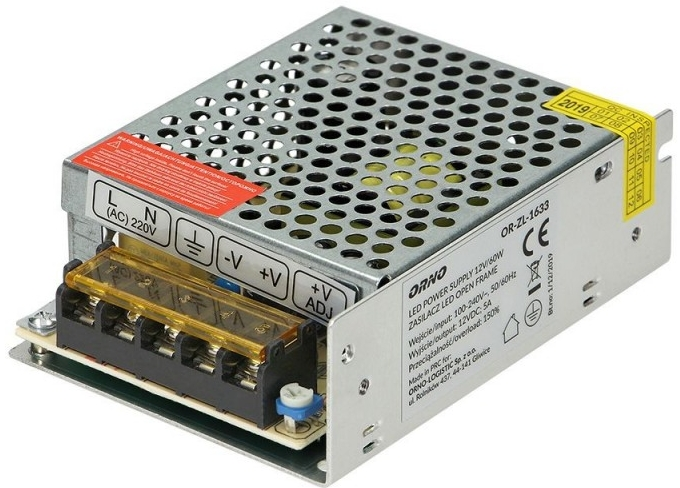
\includegraphics[width=0.5\textwidth]{07hw_specification/power_supply}
	\caption{ORNO Industrial Power Supply 12 V / 5 A.}
	\label{fig:power_supply}
\end{figure}

\paragraph*{Characteristics}
\begin{itemize}
	\item Input voltage: 100-240 V \ac{ac}, 60 W;
	\item Output voltage: 12 V \ac{dc};
	\item Output current: 5 A;
	\item Protected against overload, short circuit, over-voltage and over-heating.
\end{itemize}

\begin{table}[H]
	\centering
	\begin{tabular}{|m{5cm}|m{6cm}|}
		\hline
		\textbf{Power Supply Pinout} & \textbf{Description}
		\\\hline\hline
		 
		L & Power grid phase 230 V \ac{ac}
		\\\hline
		N & Power grid neutral
		\\\hline
		GND & GND
		\\\hline
		-V & Output -12 V \ac{dc}
		\\\hline
		+V & Output +12 V \ac{dc}
		\\\hline
	\end{tabular}
	\caption{Power Supply Pinout Description.}
	\label{table:power_supply_pinout}
\end{table}

For educational purposes, in this project the power supply will be connected to a power plug, and not directly connected with eletrical grid wires, being for that necessary a plug to bare end wire, as the one shown in figure \ref{fig:eletrical_wire}.

\begin{figure}[H]
	\centering
	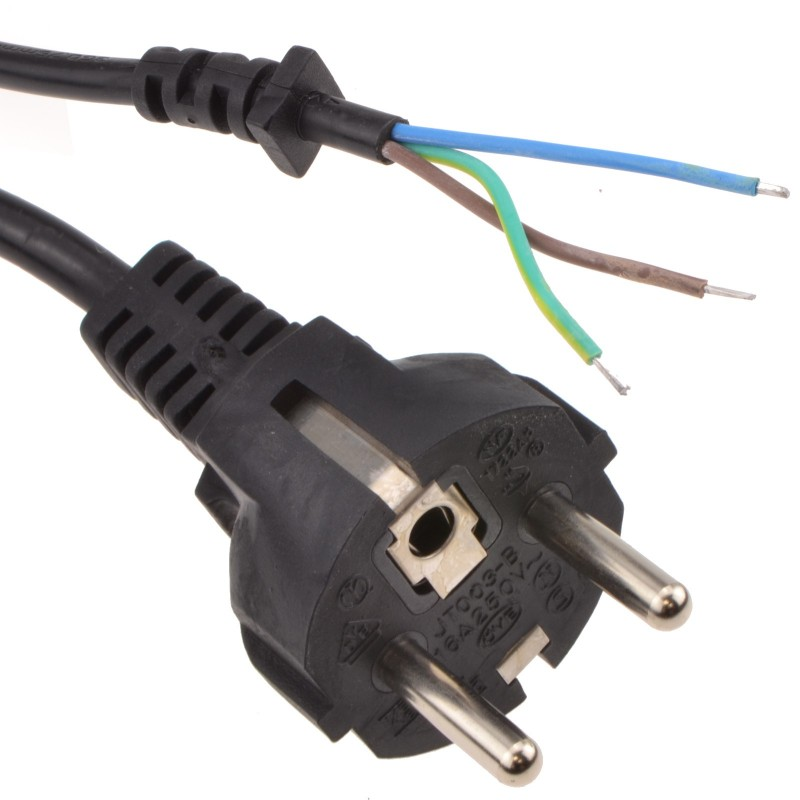
\includegraphics[width=0.4\textwidth]{07hw_specification/eletrical_wire}
	\caption{Plug to bare end wire 5 A.}
	\label{fig:eletrical_wire}
\end{figure}

The plug separates in three wires, which must be carefully connected to the power supply, as previously seen. These wires have a color pattern, as one shows in table \ref{table:color_pattern_wire}.

\begin{table}[H]
	\centering
	\begin{tabular}{|m{5cm}|m{6cm}|}
		\hline
		\textbf{Color pattern} & \textbf{Description}
		\\\hline\hline
		
		Brown wire & Power grid phase 230 V \ac{ac}
		\\\hline
		Blue wire & Power grid neutral
		\\\hline
		Green/Yellow wire & GND
		\\\hline
	\end{tabular}
	\caption{Color pattern on eletrical wires.}
	\label{table:color_pattern_wire}
\end{table}

In order to provide a lower voltage to power the Raspberry Pi and sensors, it is necessary to use a step down module, as the one shown in figure \ref{fig:step_down}, which can convert 12 V \ac{dc} to 5 V \ac{dc}. \cite{step_down}
 
\begin{figure}[H]
	\centering
	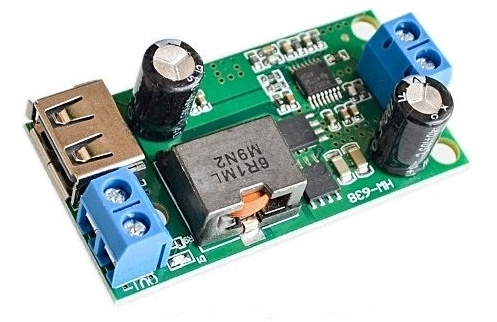
\includegraphics[width=0.5\textwidth]{07hw_specification/step_down}
	\caption{Step Down 9-38~V to 5~V / 5~A.}
	\label{fig:step_down}
\end{figure}

\paragraph*{Characteristics}
\begin{itemize}
	\item Input voltage 9-38 V;
	\item Output voltage 5 V / 5 A;
	\item Load capacity: 5 A;
	\item Maximum efficiency of 95 \%.
\end{itemize}

\begin{table}[H]
	\centering
	\begin{threeparttable}
	\begin{tabular}{|m{5cm}|m{6cm}|}
		\hline
		\textbf{Step Down Pinout} & \textbf{Description}
		\\\hline\hline
		
		VCC & Input voltage 9-38 V
		\\\hline
		GND & Input GND
		\\\hline
		USB & USB output 5 V / 5 A \tnote{*}
		\\\hline
		VOUT+ & Output 5 V / 5 A \tnote{*}
		\\\hline
		VOUT- & Output GND
		\\\hline
	\end{tabular}
	
	\begin{tablenotes}
		\small
		\item[*] This module provides 5 A for both output pins combined (USB and VOUT+).
	\end{tablenotes}
	\end{threeparttable}
	\caption{Step-Down Pinout Description.}
	\label{table:step_down_pinout}
\end{table}

\myparagraph{Connection scheme}
In table \ref{table:step_down_pinout} is shown the connection scheme for the step down. Keep in mind that the same power supply output 12 V \ac{dc} is connected directly to the lamp VCC and to the step down VCC.

\begin{table}[H]
	\centering
	\begin{tabular}{|m{5cm}|m{6cm}|}
		\hline
		\textbf{Step Down Pin} & \textbf{Connects to}
		\\\hline\hline
		
		VCC & Power supply Output +12 V \ac{dc}
		\\\hline
		GND & Power supply Output GND
		\\\hline
		USB & Raspberry Pi USB-C
		\\\hline
		VOUT+ & Sensors VCC
		\\\hline
		VOUT- & Sensors GND
		\\\hline
	\end{tabular}
	
	\caption{Connection scheme: Step Down.}
	\label{table:connect_power}
\end{table}

\myparagraph{Test Cases}
It is important to know how the step down works, and how it will behave upon certain events. In table \ref{table:test_step_down} are shown test cases to this module.

\begin{table}[H]
	\centering
	\resizebox{\columnwidth}{!}
	{
		\begin{tabular}{|m{3cm}|m{5cm}||m{5cm}|}
			\hline
			\textbf{Test Case} & \textbf{Expected Output} & \textbf{Real Output}
			\\\hline\hline
			Connect power supply to the power grid & Provide 12 V \ac{dc} & -
			\\\hline
			Connect step down to the power supply & Provide 5 V \ac{dc} & -
			\\\hline
		\end{tabular}
	}
	\caption{Test Cases: Step Down.}
	\label{table:test_step_down}
\end{table}
%**********************************************************
\subsection{Driver}
In order to control the lamp brightness through a GPIO pin from the Raspberry Pi, it's needed a driver circuit, as shown in figure \ref{fig:driver}. This circuit takes as input a \ac{pwm} signal, provided by the raspberry Pi, and also the power for the lamp, \(V_{CL}\), which comes directly from the power supply 12 V \ac{dc} output of the power module. The output of this circuit, the lamp voltage \(V_{L}\), is directly related to it's brightness, which one wants to control.

\begin{figure}[H]
	\centering
	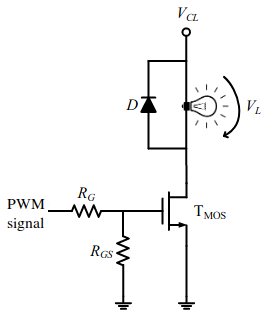
\includegraphics[width=0.5\textwidth]{07hw_specification/driver}
	\caption{Driver circuit to control lamp brightness.}
	\label{fig:driver}
\end{figure}

The \ac{pwm} signal only takes two values, 0 or 3,3 V, but its average value over time is varied, changing at high frequency the time intervals in which the transistor \(T_{MOS}\) is conducting (applied voltage 3,3 V) and at cutoff (applied voltage 0 V). So, as the \ac{pwm} duty cycle increases, the transistor conducts for more time, leading to an increase of \(V_{L}\), and, therefore, to an increase of the lamp brightness. In any case, the power dissipation in the transistor is very low, because of the rapid change between each transistor state, conducting (at saturation) or at cutoff.

\paragraph*{Characteristics}
\begin{itemize}
	\item Transistor MOSFET;
	\item Resistor \(R_{G}\) limits the current in the gate of the transistor;
	\item Resistor \(R_{GS}\) ensures that the gate is set to 0 potential when the circuit is turned off;
	\item Diode D, known as free-wheeling, provides a way to discharge the energy stored in the magnetic field of the inductive load, when the transistor turns off. For that reason, this diode must be fast;
\end{itemize}

In order to specify the components to be used, the following must be taken into account.

The temperature of the transistor (internal at the junction) must not exceed the maximum allowed by the manufacturer (typically 150 °C as in the case of STP60NF06, BUK453, BUZ90). In order for the transistor to be used without a heatsink, the internally dissipated power must not exceed 2~W (taking into account the typical thermal resistance of a TO-220 package, 60~°C/W and the ambient temperature of 30 °C). Considering that 50 \% of losses occur in conduction and 50  \% in switching (very vague approximation), the transistor can only dissipate 1 W in conduction and 1 W in switching. For an \(I_{DS}\) current of 2 A, the internal resistance (\(R_{DS}\) of MOSFET to \(V_{GS}\) voltage, \(I_{DS}\) current and operating temperature) will be a maximum of 250 m$\Omega$ (P = \(R_{DS}\).\(I_{DS2}\)).

Diode D should be fast and the MR852 is recommended.\linebreak

With this in mind, one can select the following components for the driver, as presented in table \ref{table:driver_components}.

\begin{table}[H]
	\centering
	\resizebox{\columnwidth}{!}
	{
		\begin{tabular}{|m{5cm}|m{6cm}|m{2.6cm}|}
			\hline
			\textbf{Driver Component} & \textbf{Product Name} & \textbf{Product Qty}
			\\\hline\hline
			
			\(T_{MOS}\) & BUK453 & 1
			\\\hline
			Diode D & MR852 & 1
			\\\hline
			Resistor \(R_{G}\) & Common; +-5 \% tolerance & 1
			\\\hline
			Resistor \(R_{GS}\) & Common; +-5 \% tolerance & 1
			\\\hline
		\end{tabular}
	}
	\caption{Driver components.}
	\label{table:driver_components}
\end{table}

\myparagraph{Connection scheme}
In table \ref{table:connect_driver} is shown the connection scheme for the driver circuit. (Remember figure \ref{fig:rasp_pinout} and table \ref{table:power_supply_pinout})

\begin{table}[H]
	\centering
	\begin{tabular}{|m{5cm}|m{6cm}|}
		\hline
		\textbf{Driver} & \textbf{Connects to}
		\\\hline\hline
		
		PWM Signal & Raspberry Pi PWMxxx Pinyyy
		\\\hline
		\(V_{CL}\) & Power supply Output +12 V \ac{dc}
		\\\hline
		GND & Power supply Output GND
		\\\hline
	\end{tabular}
	
	\caption{Connection scheme: Driver.}
	\label{table:connect_driver}
\end{table}

\myparagraph{Test Cases}
It is important to know how the driver works, and how it will behave upon certain events. In table \ref{table:test_driver} are shown test cases to this circuit.

\begin{table}[H]
	\centering
	\resizebox{\columnwidth}{!}
	{
		\begin{tabular}{|m{3cm}|m{5cm}||m{5cm}|}
			\hline
			\textbf{Test Case} & \textbf{Expected Output} & \textbf{Real Output}
			\\\hline\hline
			Apply 3,3 V to the transistor & Lamp at maximum bright & -
			\\\hline
			Apply 0 V to the transistor & Lamp off & -
			\\\hline
			Change \ac{pwm} signal & Variable lamp brightness & -
			\\\hline
		\end{tabular}
	}
	\caption{Test Cases: Driver.}
	\label{table:test_driver}
\end{table}

%**********************************************************
\subsection{Hardware review} %?????
% show hardware architecture with all protocols defined in
% each connection